\documentclass[11pt]{article}
\usepackage{cornell-notes}
\usepackage{mathtools}
\usepackage{needspace}
\usepackage{ragged2e}
\usepackage{adjustbox}
\usepackage{tikz}
\usetikzlibrary{arrows.meta,positioning}
\tcbuselibrary{most}
\geometry{letterpaper,margin=0.72in,headheight=15pt}
\setCornellCollection{Calculus Cornell Notes}
\setCornellUnitType{Chapter}
\setCornellUnitNumber{8}
\setCornellUnitTitle{Integration Techniques and Improper Integrals}

\definecolor{Ink}{HTML}{17324D}
\definecolor{Teal}{HTML}{147D78}
\definecolor{Sky}{HTML}{DDEEF1}
\definecolor{Cue}{HTML}{EEF2F5}
\definecolor{Warm}{HTML}{FFF3D6}
\definecolor{Alert}{HTML}{9D3C32}
\definecolor{Green}{HTML}{276749}
\definecolor{Rule}{HTML}{AAB8C2}
\hypersetup{colorlinks=true,linkcolor=Ink,urlcolor=Teal,pdfborder={0 0 0}}
\setlength{\parindent}{0pt}
\setlength{\parskip}{4pt}
\setlist{nosep,leftmargin=*}
\titleformat{\section}{\Large\bfseries\color{Ink}}{}{0pt}{}[\color{Teal}\titlerule]
\titleformat{\subsection}{\large\bfseries\color{Teal}}{}{0pt}{}
\pagestyle{fancy}
\fancyhf{}
\fancyhead[L]{\small\color{Ink}\textsc{Cornell Notes}}
\fancyhead[R]{\small\color{Teal}\nouppercase{\leftmark}}
\fancyfoot[L]{\footnotesize\color{Ink}Active recall $\bullet$ Worked reasoning $\bullet$ Verification}
\fancyfoot[R]{\footnotesize\color{Ink}\thepage\ of \pageref*{LastPage}}
\renewcommand{\headrulewidth}{0.5pt}
\renewcommand{\footrulewidth}{0.4pt}
\newcolumntype{Y}{>{\RaggedRight\arraybackslash}X}
\newtcolorbox{orientationbox}{enhanced,breakable,colback=Sky,colframe=Teal,boxrule=0.7pt,arc=2mm,title=Chapter orientation,fonttitle=\bfseries}
\newtcolorbox{sectionsummarybox}{enhanced,breakable,colback=white,colframe=Teal,boxrule=0.6pt,arc=1.5mm,left=2mm,right=2mm,top=1mm,bottom=1mm,title=Section synthesis,fonttitle=\bfseries\color{Teal}}
\newtcolorbox{warningbox}{enhanced,breakable,colback=Warm,colframe=Alert,boxrule=0.7pt,arc=1.5mm,title=Common error audit,fonttitle=\bfseries}
\newtcolorbox{checkbox}{enhanced,breakable,colback=white,colframe=Green,boxrule=0.7pt,arc=1.5mm,title=Verification habit,fonttitle=\bfseries}
\newcommand{\cornellcuehead}{\rowcolor{Ink}\color{white}\bfseries Cue / recall prompt & \color{white}\bfseries Notes / reasoning \\\endhead}
\newcommand{\cornellcuerow}[2]{\rowcolor{Cue}#1 & #2 \\\addlinespace[3pt]}
% Table-safe: delegates to the shared Cornell formula box (cornell-notes.sty),
% which cannot emit \pagebreak/\noalign inside longtable cells.
\newcommand{\formula}[1]{\CornellFormula[colback=Sky,colframe=Teal]{#1}}

\title{Chapter 8: Integration Techniques and Improper Integrals\\[2mm]\large Cornell Notes}
\author{}
\date{}
\hypersetup{pdftitle={Chapter 8: Integration Techniques and Improper Integrals - Cornell Notes},pdfauthor={},pdfsubject={Calculus study notes},pdfkeywords={calculus, Cornell notes, active recall}}
\begin{document}
\maketitle
\thispagestyle{fancy}
\begin{orientationbox}
Select and verify advanced integration methods, approximate definite integrals, and interpret unbounded integrals through limits. These notes follow the complete local section sequence (515--586) and emphasize definitions, governing results, strategy selection, and verifiable reasoning.
\end{orientationbox}

\section{Prerequisite map}
\begin{minipage}[t]{0.42\textwidth}
\textbf{Bring forward}
\begin{itemize}
\item Substitution
\item Trigonometric identities
\item Algebraic decomposition
\item Limits
\end{itemize}
\end{minipage}\hfill
\begin{minipage}[t]{0.54\textwidth}
\textbf{Chapter flow}
\begin{center}
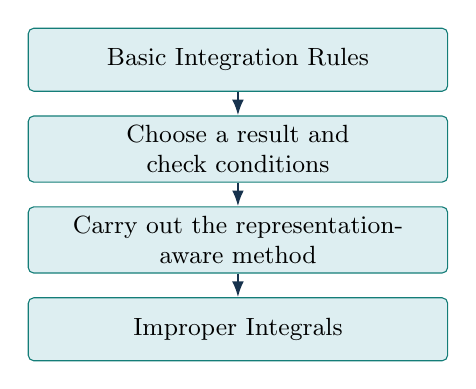
\begin{tikzpicture}[node distance=3mm, every node/.style={font=\small,align=center}, box/.style={draw=Teal,rounded corners=2pt,fill=Sky,minimum height=8mm,text width=0.42\textwidth}, arr/.style={-{Latex[length=2mm]},thick,draw=Ink}]
\node[box] (a) {Basic Integration Rules};
\node[box,below=of a] (b) {Choose a result and check conditions};
\node[box,below=of b] (c) {Carry out the representation-aware method};
\node[box,below=of c] (d) {Improper Integrals};
\draw[arr] (a)--(b); \draw[arr] (b)--(c); \draw[arr] (c)--(d);
\end{tikzpicture}
\end{center}
\end{minipage}

\section{Learning objectives}
\begin{enumerate}
\item Explain the central objects and hypotheses in 8.1 and 8.8.
\item Translate among algebraic, graphical, numerical, and verbal representations.
\item Select an appropriate formula or theorem before beginning symbolic work.
\item Carry out multi-step calculations while preserving domain, sign, orientation, and units.
\item Diagnose common errors by testing assumptions and checking the result independently.
\item Synthesize the chapter's methods into a reusable problem-solving workflow.
\end{enumerate}

\section{8.1 Basic Integration Rules}
\begin{longtable}{C N}\cornellcuehead
\cornellcuerow{What is the governing idea in 8.1?}{Integration strategy starts by simplifying algebra and recognizing standard antiderivative patterns.}
\cornellcuerow{Which result should be recalled?}{\formula{\int [af(x)+bg(x)]dx=a\int f+b\int g}}
\cornellcuerow{How should a problem be organized?}{Rewrite powers and fractions, separate sums, factor constants, match a rule, and differentiate the result.}
\cornellcuerow{What should be checked before accepting an answer?}{Confirm the hypotheses and domain, preserve units and orientation when relevant, and substitute or differentiate back into the defining relation.}
\end{longtable}
\begin{warningbox}Linearity does not permit splitting products or quotients into separate integrals.\end{warningbox}
\begin{sectionsummarybox}Integration strategy starts by simplifying algebra and recognizing standard antiderivative patterns. The operational habit is to rewrite powers and fractions, separate sums, factor constants, match a rule, and differentiate the result.\end{sectionsummarybox}
\section{8.2 Integration by Parts}
\begin{longtable}{C N}\cornellcuehead
\cornellcuerow{What is the governing idea in 8.2?}{Integration by parts reverses the product rule and transfers differentiation to a strategically chosen factor.}
\cornellcuerow{Which result should be recalled?}{\formula{\int u\,dv=uv-\int v\,du}}
\cornellcuerow{How should a problem be organized?}{Choose $u$ to simplify under differentiation, compute $dv$ completely, and repeat or solve algebraically when the original integral returns.}
\cornellcuerow{What should be checked before accepting an answer?}{Confirm the hypotheses and domain, preserve units and orientation when relevant, and substitute or differentiate back into the defining relation.}
\end{longtable}
\begin{warningbox}Failing to integrate $dv$, losing the minus sign, or choosing a more complicated $du$ creates extra work.\end{warningbox}
\begin{sectionsummarybox}Integration by parts reverses the product rule and transfers differentiation to a strategically chosen factor. The operational habit is to choose $u$ to simplify under differentiation, compute $dv$ completely, and repeat or solve algebraically when the original integral returns.\end{sectionsummarybox}
\section{8.3 Trigonometric Integrals}
\begin{longtable}{C N}\cornellcuehead
\cornellcuerow{What is the governing idea in 8.3?}{Powers and products of trigonometric functions are reduced using parity patterns and identities.}
\cornellcuerow{Which result should be recalled?}{\formula{\sin^2x+\cos^2x=1,\qquad \sec^2x=1+\tan^2x}}
\cornellcuerow{How should a problem be organized?}{Classify the powers, save a factor suited to substitution when one exponent is odd, and use power-reduction identities when both are even.}
\cornellcuerow{What should be checked before accepting an answer?}{Confirm the hypotheses and domain, preserve units and orientation when relevant, and substitute or differentiate back into the defining relation.}
\end{longtable}
\begin{warningbox}Applying an identity without matching its sign or parity case can make the integrand harder.\end{warningbox}
\begin{sectionsummarybox}Powers and products of trigonometric functions are reduced using parity patterns and identities. The operational habit is to classify the powers, save a factor suited to substitution when one exponent is odd, and use power-reduction identities when both are even.\end{sectionsummarybox}
\section{8.4 Trigonometric Substitution}
\begin{longtable}{C N}\cornellcuehead
\cornellcuerow{What is the governing idea in 8.4?}{Radicals involving quadratic forms become trigonometric identities under geometry-matched substitutions.}
\cornellcuerow{Which result should be recalled?}{\formula{\sqrt{a^2-x^2}:\ x=a\sin\theta;\quad \sqrt{a^2+x^2}:\ x=a\tan\theta}}
\cornellcuerow{How should a problem be organized?}{Match the radical, substitute $x$ and $dx$, simplify with the intended identity, integrate in $	heta$, and return using a reference triangle.}
\cornellcuerow{What should be checked before accepting an answer?}{Confirm the hypotheses and domain, preserve units and orientation when relevant, and substitute or differentiate back into the defining relation.}
\end{longtable}
\begin{warningbox}Choosing a substitution with the wrong identity or ignoring the angle range causes sign errors in radicals.\end{warningbox}
\begin{sectionsummarybox}Radicals involving quadratic forms become trigonometric identities under geometry-matched substitutions. The operational habit is to match the radical, substitute $x$ and $dx$, simplify with the intended identity, integrate in $	heta$, and return using a reference triangle.\end{sectionsummarybox}
\section{8.5 Partial Fractions}
\begin{longtable}{C N}\cornellcuehead
\cornellcuerow{What is the governing idea in 8.5?}{A proper rational function decomposes into simpler fractions determined by the factorization and multiplicity of its denominator.}
\cornellcuerow{Which result should be recalled?}{\formula{\frac{P(x)}{Q(x)}=\sum\frac{A}{(x-a)^k}+\sum\frac{Bx+C}{(x^2+bx+c)^k}}}
\cornellcuerow{How should a problem be organized?}{Divide first if improper, factor over the reals, write every required term, solve coefficients, then integrate the pieces.}
\cornellcuerow{What should be checked before accepting an answer?}{Confirm the hypotheses and domain, preserve units and orientation when relevant, and substitute or differentiate back into the defining relation.}
\end{longtable}
\begin{warningbox}Missing repeated-factor terms or using a constant numerator over an irreducible quadratic makes the decomposition incomplete.\end{warningbox}
\begin{sectionsummarybox}A proper rational function decomposes into simpler fractions determined by the factorization and multiplicity of its denominator. The operational habit is to divide first if improper, factor over the reals, write every required term, solve coefficients, then integrate the pieces.\end{sectionsummarybox}
\section{8.6 Numerical Integration}
\begin{longtable}{C N}\cornellcuehead
\cornellcuerow{What is the governing idea in 8.6?}{Trapezoidal and Simpson rules approximate accumulation from sampled values with method-specific weights and error behavior.}
\cornellcuerow{Which result should be recalled?}{\formula{T_n=\frac{\Delta x}{2}[f_0+2f_1+\cdots+2f_{n-1}+f_n]}}
\cornellcuerow{How should a problem be organized?}{Use equally spaced nodes, apply the correct weight pattern, ensure Simpson's $n$ is even, and compare refinements when possible.}
\cornellcuerow{What should be checked before accepting an answer?}{Confirm the hypotheses and domain, preserve units and orientation when relevant, and substitute or differentiate back into the defining relation.}
\end{longtable}
\begin{warningbox}Confusing the number of subintervals with the number of sample points shifts $\Delta x$ and the weights.\end{warningbox}
\begin{sectionsummarybox}Trapezoidal and Simpson rules approximate accumulation from sampled values with method-specific weights and error behavior. The operational habit is to use equally spaced nodes, apply the correct weight pattern, ensure Simpson's $n$ is even, and compare refinements when possible.\end{sectionsummarybox}
\section{8.7 Integration by Tables and Other Integration Techniques}
\begin{longtable}{C N}\cornellcuehead
\cornellcuerow{What is the governing idea in 8.7?}{A table entry is a pattern that may require algebra, substitution, or parameter matching before it applies.}
\cornellcuerow{Which result should be recalled?}{\formula{\int f(ax+b)\,dx=\frac1aF(ax+b)+C}}
\cornellcuerow{How should a problem be organized?}{Normalize the integrand to a listed form, map every parameter, include scale factors, and verify by differentiation.}
\cornellcuerow{What should be checked before accepting an answer?}{Confirm the hypotheses and domain, preserve units and orientation when relevant, and substitute or differentiate back into the defining relation.}
\end{longtable}
\begin{warningbox}Visual resemblance without exact parameter matching is not enough to justify a table formula.\end{warningbox}
\begin{sectionsummarybox}A table entry is a pattern that may require algebra, substitution, or parameter matching before it applies. The operational habit is to normalize the integrand to a listed form, map every parameter, include scale factors, and verify by differentiation.\end{sectionsummarybox}
\section{8.8 Improper Integrals}
\begin{longtable}{C N}\cornellcuehead
\cornellcuerow{What is the governing idea in 8.8?}{An unbounded interval or integrand is defined by one-sided limits of proper integrals; convergence is a finite-limit property.}
\cornellcuerow{Which result should be recalled?}{\formula{\int_a^{\infty}f=\lim_{b\to\infty}\int_a^b f}}
\cornellcuerow{How should a problem be organized?}{Locate every improper endpoint, split at interior singularities, evaluate each one-sided limit separately, and declare convergence only if all are finite.}
\cornellcuerow{What should be checked before accepting an answer?}{Confirm the hypotheses and domain, preserve units and orientation when relevant, and substitute or differentiate back into the defining relation.}
\end{longtable}
\begin{warningbox}Cancellation across a singularity does not make the standard improper integral converge.\end{warningbox}
\begin{sectionsummarybox}An unbounded interval or integrand is defined by one-sided limits of proper integrals; convergence is a finite-limit property. The operational habit is to locate every improper endpoint, split at interior singularities, evaluate each one-sided limit separately, and declare convergence only if all are finite.\end{sectionsummarybox}

\section{Definitions and theorem register}
\small
\begin{longtable}{@{}>{\RaggedRight\arraybackslash}p{0.24\textwidth}>{\RaggedRight\arraybackslash}p{0.40\textwidth}>{\RaggedRight\arraybackslash}p{0.29\textwidth}@{}}
\toprule
\textbf{Topic} & \textbf{Meaning and conditions} & \textbf{Canonical form}\\
\midrule\endhead
8.1 Basic Integration Rules & Integration strategy starts by simplifying algebra and recognizing standard antiderivative patterns. & \adjustbox{max width=\linewidth}{\(\displaystyle \int [af(x)+bg(x)]dx=a\int f+b\int g\)} \\\addlinespace[2pt]
8.2 Integration by Parts & Integration by parts reverses the product rule and transfers differentiation to a strategically chosen factor. & \adjustbox{max width=\linewidth}{\(\displaystyle \int u\,dv=uv-\int v\,du\)} \\\addlinespace[2pt]
8.3 Trigonometric Integrals & Powers and products of trigonometric functions are reduced using parity patterns and identities. & \adjustbox{max width=\linewidth}{\(\displaystyle \sin^2x+\cos^2x=1,\qquad \sec^2x=1+\tan^2x\)} \\\addlinespace[2pt]
8.4 Trigonometric Substitution & Radicals involving quadratic forms become trigonometric identities under geometry-matched substitutions. & \adjustbox{max width=\linewidth}{\(\displaystyle \sqrt{a^2-x^2}:\ x=a\sin\theta;\quad \sqrt{a^2+x^2}:\ x=a\tan\theta\)} \\\addlinespace[2pt]
8.5 Partial Fractions & A proper rational function decomposes into simpler fractions determined by the factorization and multiplicity of its denominator. & \adjustbox{max width=\linewidth}{\(\displaystyle \frac{P(x)}{Q(x)}=\sum\frac{A}{(x-a)^k}+\sum\frac{Bx+C}{(x^2+bx+c)^k}\)} \\\addlinespace[2pt]
8.6 Numerical Integration & Trapezoidal and Simpson rules approximate accumulation from sampled values with method-specific weights and error behavior. & \adjustbox{max width=\linewidth}{\(\displaystyle T_n=\frac{\Delta x}{2}[f_0+2f_1+\cdots+2f_{n-1}+f_n]\)} \\\addlinespace[2pt]
8.7 Integration by Tables and Other Integration Techniques & A table entry is a pattern that may require algebra, substitution, or parameter matching before it applies. & \adjustbox{max width=\linewidth}{\(\displaystyle \int f(ax+b)\,dx=\frac1aF(ax+b)+C\)} \\\addlinespace[2pt]
8.8 Improper Integrals & An unbounded interval or integrand is defined by one-sided limits of proper integrals; convergence is a finite-limit property. & \adjustbox{max width=\linewidth}{\(\displaystyle \int_a^{\infty}f=\lim_{b\to\infty}\int_a^b f\)} \\\addlinespace[2pt]
\bottomrule
\end{longtable}
\normalsize

\section{Formula and method sheet}
\small
\begin{longtable}{@{}>{\RaggedRight\arraybackslash}p{0.08\textwidth}>{\RaggedRight\arraybackslash}p{0.48\textwidth}>{\RaggedRight\arraybackslash}p{0.37\textwidth}@{}}
\toprule
\textbf{Sec.} & \textbf{Method sequence} & \textbf{Stop-and-check trigger}\\
\midrule\endhead
8.1 & Rewrite powers and fractions, separate sums, factor constants, match a rule, and differentiate the result. & Linearity does not permit splitting products or quotients into separate integrals. \\\addlinespace[2pt]
8.2 & Choose $u$ to simplify under differentiation, compute $dv$ completely, and repeat or solve algebraically when the original integral returns. & Failing to integrate $dv$, losing the minus sign, or choosing a more complicated $du$ creates extra work. \\\addlinespace[2pt]
8.3 & Classify the powers, save a factor suited to substitution when one exponent is odd, and use power-reduction identities when both are even. & Applying an identity without matching its sign or parity case can make the integrand harder. \\\addlinespace[2pt]
8.4 & Match the radical, substitute $x$ and $dx$, simplify with the intended identity, integrate in $ heta$, and return using a reference triangle. & Choosing a substitution with the wrong identity or ignoring the angle range causes sign errors in radicals. \\\addlinespace[2pt]
8.5 & Divide first if improper, factor over the reals, write every required term, solve coefficients, then integrate the pieces. & Missing repeated-factor terms or using a constant numerator over an irreducible quadratic makes the decomposition. \\\addlinespace[2pt]
8.6 & Use equally spaced nodes, apply the correct weight pattern, ensure Simpson's $n$ is even, and compare refinements when possible. & Confusing the number of subintervals with the number of sample points shifts $\Delta x$ and the weights. \\\addlinespace[2pt]
8.7 & Normalize the integrand to a listed form, map every parameter, include scale factors, and verify by differentiation. & Visual resemblance without exact parameter matching is not enough to justify a table formula. \\\addlinespace[2pt]
8.8 & Locate every improper endpoint, split at interior singularities, evaluate each one-sided limit separately, and declare convergence only if all are. & Cancellation across a singularity does not make the standard improper integral converge. \\\addlinespace[2pt]
\bottomrule
\end{longtable}
\normalsize

\section{Common errors and diagnostic checks}
\begin{warningbox}
\begin{itemize}
\item \textbf{8.1:} Linearity does not permit splitting products or quotients into separate integrals.
\item \textbf{8.2:} Failing to integrate $dv$, losing the minus sign, or choosing a more complicated $du$ creates extra work.
\item \textbf{8.3:} Applying an identity without matching its sign or parity case can make the integrand harder.
\item \textbf{8.4:} Choosing a substitution with the wrong identity or ignoring the angle range causes sign errors in radicals.
\item \textbf{8.5:} Missing repeated-factor terms or using a constant numerator over an irreducible quadratic makes the decomposition incomplete.
\item \textbf{8.6:} Confusing the number of subintervals with the number of sample points shifts $\Delta x$ and the weights.
\item \textbf{8.7:} Visual resemblance without exact parameter matching is not enough to justify a table formula.
\item \textbf{8.8:} Cancellation across a singularity does not make the standard improper integral converge.
\end{itemize}
\end{warningbox}
\begin{checkbox}
Before accepting any result: state the relevant domain; check theorem hypotheses; estimate sign and scale; preserve units and orientation; and verify by substitution, differentiation, a limiting case, or a second representation.
\end{checkbox}

\section{Chapter synthesis}
Select and verify advanced integration methods, approximate definite integrals, and interpret unbounded integrals through limits. The chapter begins with \textbf{Basic Integration Rules} and culminates in \textbf{Improper Integrals}. Across the sequence, the most reliable workflow is to identify the mathematical object, choose a representation, state the governing result with its hypotheses, compute without dropping restrictions, and audit the answer against the original definition. Integration technique is a decision process: normalize the integrand, select a reversible transformation, preserve conditions, and verify either by differentiation or convergence limits.

\section{Self-test questions}
\begin{enumerate}
\item Explain the central distinction or object in 8.1, using both words and notation.
\item State the main formula or result from 8.2 and identify every hypothesis or restriction needed for its use.
\item Describe the problem-solving procedure for 8.3. What is the strongest independent check?
\item Compare the roles of Basic Integration Rules and Improper Integrals within this chapter.
\item Reconstruct the governing formula for 8.4 from its geometric or analytic meaning.
\item Choose one method in the chapter and explain how its output should be interpreted, including units or orientation when applicable.
\item Scenario: A student working on 8.1 produces a polished calculation but makes this error: Linearity does not permit splitting products or quotients into separate integrals. Diagnose the earliest invalid step and repair the workflow.
\item Scenario: A solution in 8.2 quotes the displayed formula without checking conditions. Which conditions must be checked, and what could fail if they are absent?
\item Construct a concept map linking a representation, a governing result, a computation, and a verification check from this chapter.
\item Design a two-part test for mastery: one conceptual prompt and one calculation. State what evidence would count as a complete answer.
\end{enumerate}

\Needspace{8\baselineskip}
\section{Answer key}
\small
\begin{enumerate}
\item A complete response identifies Integration strategy starts by simplifying algebra and recognizing standard antiderivative patterns. It should connect that meaning to \(\int [af(x)+bg(x)]dx=a\int f+b\int g\) and state the relevant domain.
\item The organizing result is \(\int u\,dv=uv-\int v\,du\). The solver must check that the quantities are defined and that the assumptions named in 8.2 hold before applying it.
\item Use this sequence: Classify the powers, save a factor suited to substitution when one exponent is odd, and use power-reduction identities when both are even. The strongest check is to return to the defining relation or differentiate/substitute the result, as appropriate.
\item Basic Integration Rules establishes integration strategy starts by simplifying algebra and recognizing standard antiderivative patterns. Improper Integrals extends the chapter to an unbounded interval or integrand is defined by one-sided limits of proper integrals; convergence is a finite-limit property. The connection is the reuse of the same representations under a broader method.
\item The formula \(\sqrt{a^2-x^2}:\ x=a\sin\theta;\quad \sqrt{a^2+x^2}:\ x=a\tan\theta\) follows by translating the defining geometric or rate relationship into symbols; each factor records a distinct change or scale.
\item Interpretation must name what varies, with respect to what, and on which domain. A numerical value without units, sign, direction, or interval information is incomplete whenever those features are part of the modeled quantity.
\item The earliest fault is the unverified assumption described by this warning: Linearity does not permit splitting products or quotients into separate integrals. Restart by following this procedure: Rewrite powers and fractions, separate sums, factor constants, match a rule, and differentiate the result.
\item The formula \(\int u\,dv=uv-\int v\,du\) is conditional, not decorative. Check domain, differentiability or integrability as relevant, boundary or orientation requirements, and nonzero denominators before drawing a conclusion.
\item One valid map is: the representation in 8.1 identifies the object; the result in 8.2 supplies a rule; the method in 8.3 carries out the computation; the check in 8.8 tests the conclusion against its definition.
\item The conceptual prompt should require explanation of a definition and its hypotheses. The calculation should require method selection rather than direct substitution. Full evidence includes setup, justified transformations, a result, and an independent check.
\end{enumerate}
\normalsize

\section{Key-term recap}
\small
\begin{longtable}{@{}>{\RaggedRight\arraybackslash}p{0.29\textwidth}>{\RaggedRight\arraybackslash}p{0.64\textwidth}@{}}
\toprule
\textbf{Term} & \textbf{Working meaning}\\
\midrule\endhead
Basic Integration Rules & Integration strategy starts by simplifying algebra and recognizing standard antiderivative patterns. \\\addlinespace[2pt]
Integration by Parts & Integration by parts reverses the product rule and transfers differentiation to a strategically chosen factor. \\\addlinespace[2pt]
Trigonometric Integrals & Powers and products of trigonometric functions are reduced using parity patterns and identities. \\\addlinespace[2pt]
Trigonometric Substitution & Radicals involving quadratic forms become trigonometric identities under geometry-matched substitutions. \\\addlinespace[2pt]
Partial Fractions & A proper rational function decomposes into simpler fractions determined by the factorization and multiplicity of its denominator. \\\addlinespace[2pt]
Numerical Integration & Trapezoidal and Simpson rules approximate accumulation from sampled values with method-specific weights and error behavior. \\\addlinespace[2pt]
Integration by Tables and Other Integration Techniques & A table entry is a pattern that may require algebra, substitution, or parameter matching before it applies. \\\addlinespace[2pt]
Improper Integrals & An unbounded interval or integrand is defined by one-sided limits of proper integrals; convergence is a finite-limit property. \\\addlinespace[2pt]
\bottomrule
\end{longtable}
\normalsize

\enlargethispage{4\baselineskip}
\begin{tcolorbox}[title=One-sentence takeaway,fonttitle=\bfseries,colback=Ink,colframe=Ink,coltext=white,coltitle=white,arc=2mm,boxrule=0pt]
\centering\bfseries Integration technique is a decision process: normalize the integrand, select a reversible transformation, preserve conditions, and verify either by differentiation or convergence limits.
\end{tcolorbox}
\end{document}
